\section{基于表面编码的对应关系剪枝}

ZebraPose\cite{su2022zebrapose} 使用\autoref{sec:hipose_encoding}所述的二进制编码从单张RGB图像中进行位姿估计。ZebraPose训练了一个神经网络来估计物体检测框内每个像素 $\bm{p}_{u,v}$ 的 $d$ 位二进制编码,从而建立像素 $\bm{p}_{u,v}$ 和物体模型的坐标 $\bm{v}_{i}$ 之间的2D-3D对应关系。其中$\bm{p}_{u,v}$表示横坐标为$u$,纵坐标为$v$的像素点。这些对应关系被提供给一个Perspective-n-Point (PnP) 求解器(例如 RANSAC+EPnP\cite{EPnP})来估计物体位姿。结果表明,这种编码的表面表示非常适合神经网络训练,避免网络直接学习一个准确的浮点数所造成的误差。

然而,这种方法:(1) 在预测对应关系阶段没有使用深度信息,(2) 没有明确利用编码表面预测的层次结构,(3) 没有利用预测表面编码的固有置信度。相反,范围 $[0,1]$ 内的连续二进制编码估计被量化为离散的位值,从而丢弃了所有置信度信息。

相比之下,本章方法 HiPose 旨在以单张 RGB-D 图像作为输入,并从彩色图像和深度图像两种模态输入中提取特征以预测 3D-3D 对应关系,如\autoref{fig:overview}所示。该框架使用RGB-D 图像的裁剪区域作为输入,并使用全流双向融合网络为目标物体上的每个点云块预测一个 $m+n$ 位的二进制编码。前 $m$ 位编码指向相对粗糙的表面(蓝线),而最后 $n$ 位编码被用作指示符,进行分层表面划分(红线)。通过迭代识别细粒度点到表面的对应关系,算法最终产生精确估计的位姿。模型上的彩色块代表不同的表面划分。最终,对于每个 3D 点 $\bm{P}$,网络被训练来预测一个二进制编码 $\hat{\bm{c}}$。该编码表示点云和物体模型之间的 3D-3D 对应关系。通过将这些对应关系传递给 Kabsch 位姿估计算法\cite{umeyama1991least},可以获得准确的位姿估计结果。

\begin{figure}[ht]
    \centering
    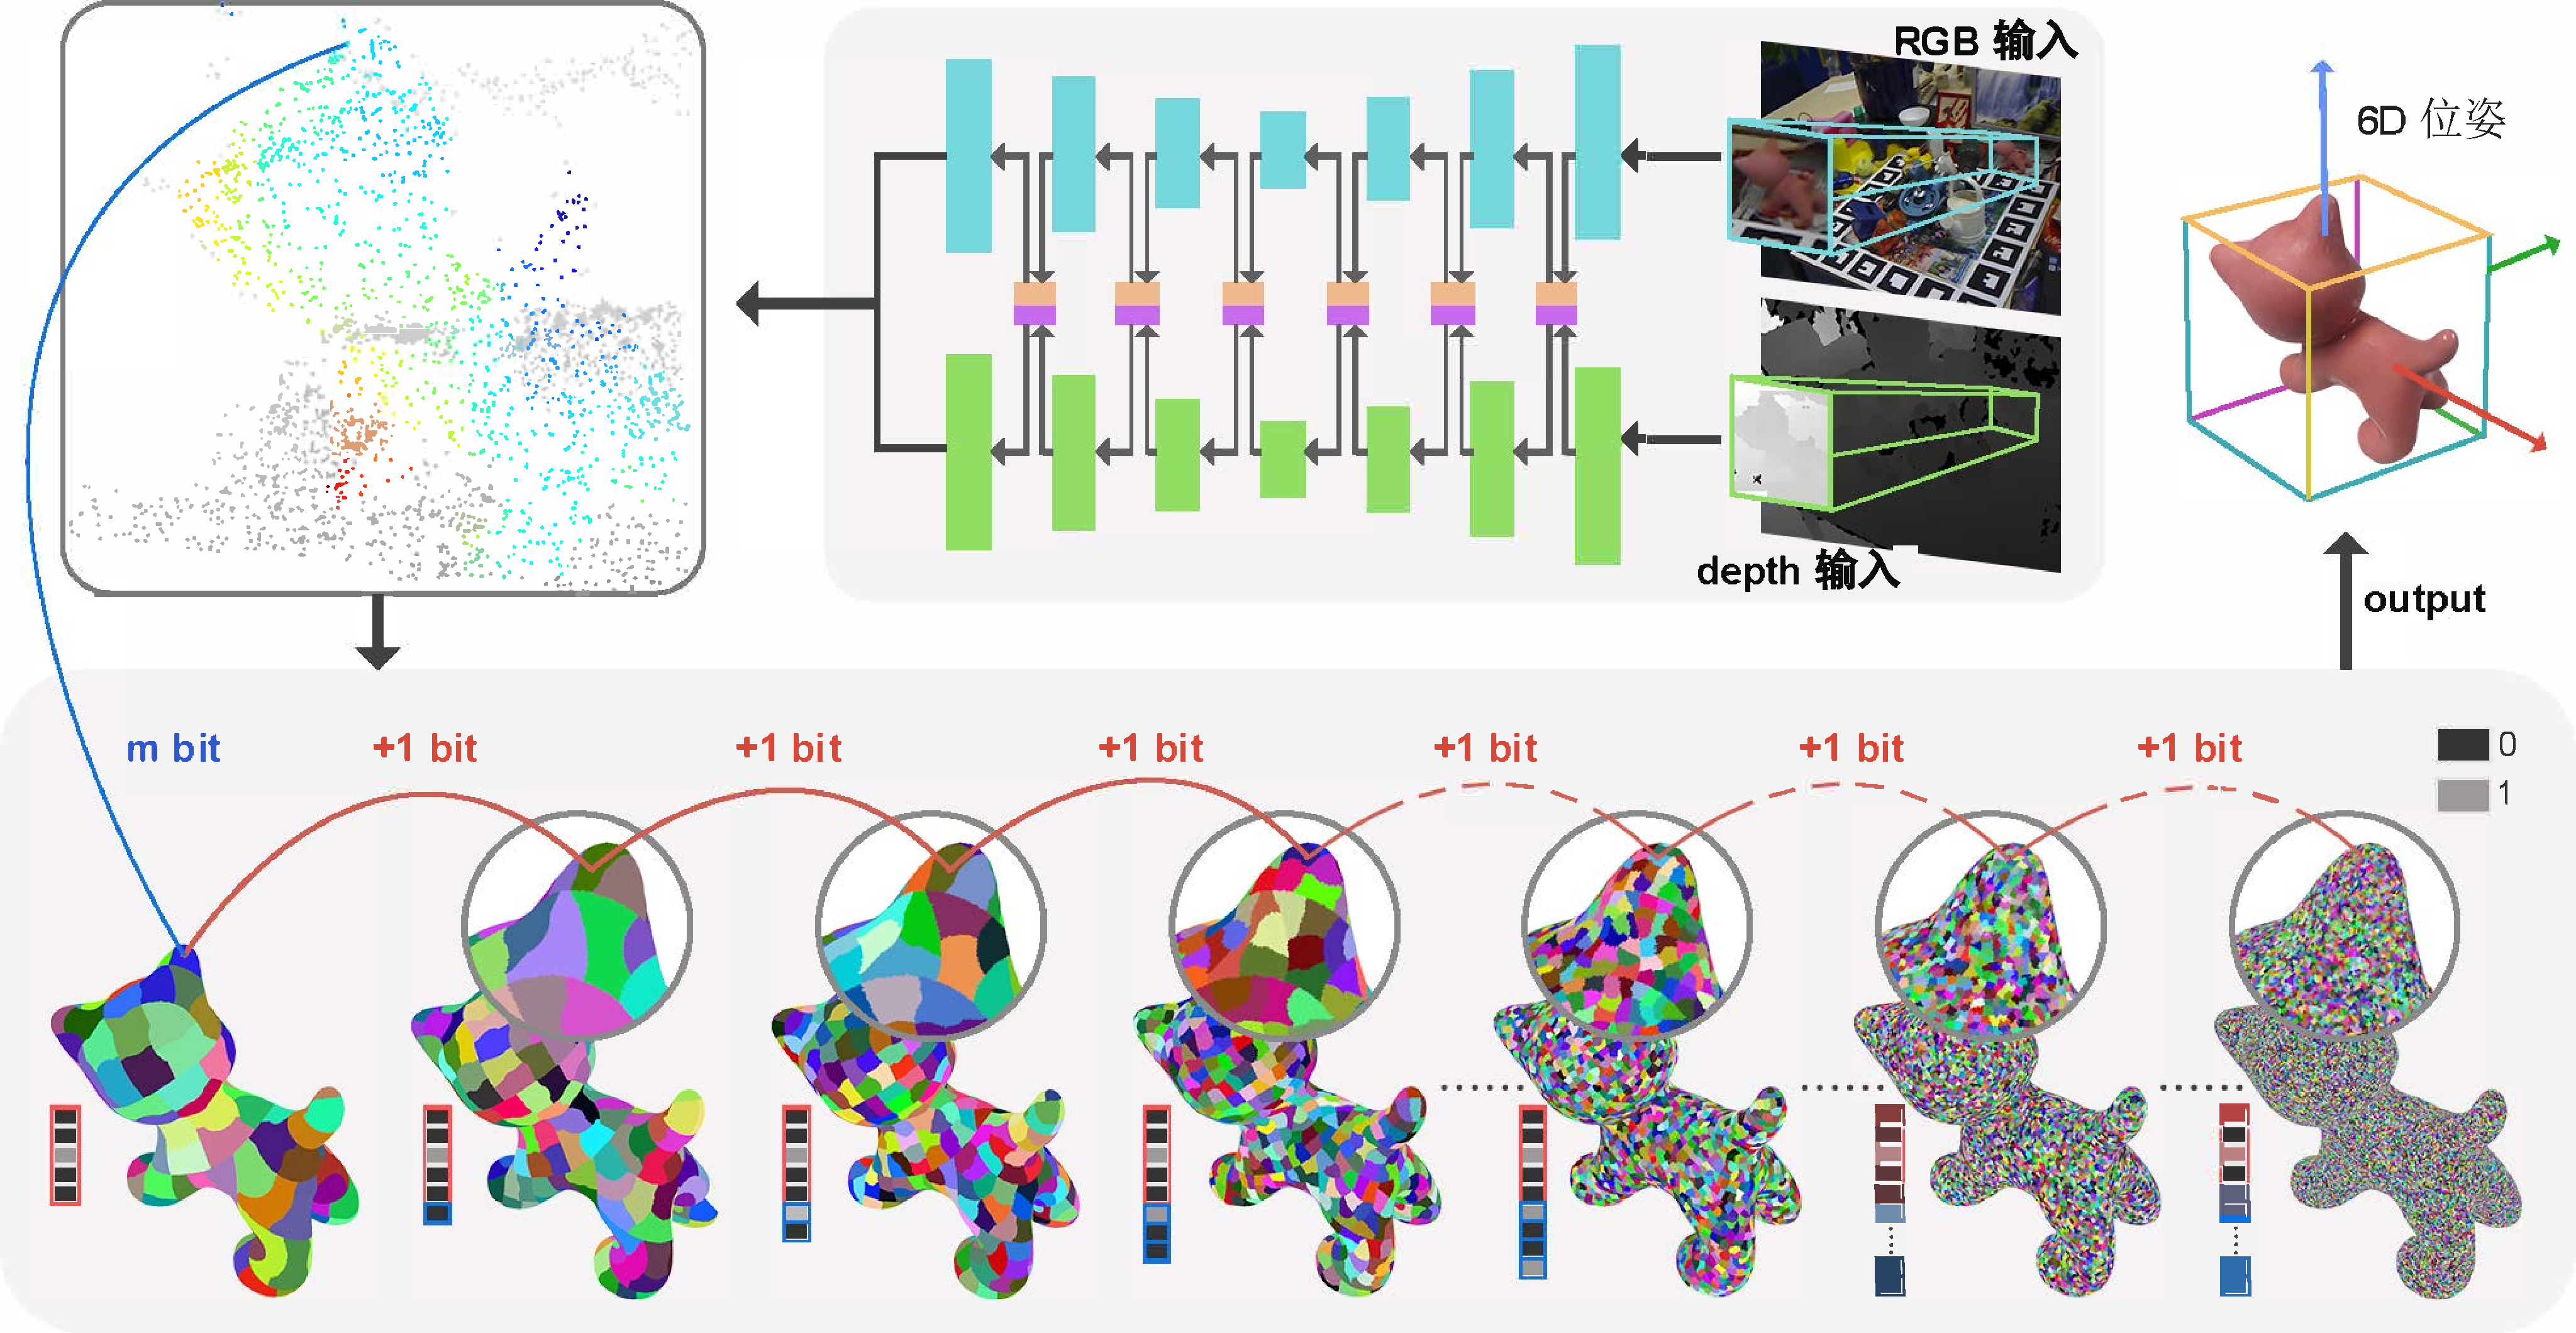
\includegraphics[width=\textwidth]{figure/hipose/overview.pdf}
    \caption{HiPose框架流程图}
    \label{fig:overview}
\end{figure}

该方法属于密集对应关系法的一种,其对二进制编码层次结构的利用催生了一种与其他密集对应关系方法不同的由粗到细的层次化处理策略。如\autoref{sec:hipose_encoding}所述,一串二进制编码表示对象表面的聚类过程,其中位数更多的二进制编码表示更多次的划分过程,而位数更高的二进制编码则表示更加细致的划分过程。HiPose 方法将二进制编码分为两组:前 $m$ 位和后 $n$ 位(共 $d=m+n$ 位)。与 ZebraPose\cite{su2022zebrapose} 不同,HiPose 并不直接处理包含最后几位高不确定性的完整编码,而是以迭代方式逐步利用第 ${m+1}$ 位到第 $d$ 位的编码信息。

对于输入点云中的某个点,编码的前 $m$ 位表示该点到物体模型表面区域$\bm{S}_{m}$的对应关系。表面区域 $\bm{S}_{m}$ 的质心点可作为模型上的3D点以创建3D-3D对应关系。然后可以从这些对应关系中估计一个粗略的位姿 $\hat{\bm{T}}_{0}$。该粗位姿将用于如\autoref{subsection:pruning} 所述的离群点去除,而剔除了离群点后的部分将使用更多位的编码收缩物体表面。以粗到细的方式迭代重复该过程,每次迭代中对应物体表面区域从 $\bm{S}_{m+1}$ 到 $\bm{S}_{m+n}$ 逐渐减小。同时,每次迭代的位姿估计精度逐步提高,并可用于更高阈值的离群值去除。

\subsection{层次化二进制编码解码}
\label{subsection:solver}
现有的方法,如 ZebraPose\cite{su2022zebrapose},直接使用预测的连续编码。神经网络输出通过sigmoid函数映射到$[0,1]$ 范围的连续估计编码,然后通过量化为位值来转换为二进制编码。然而,这种方法丢弃了预测编码中固有的置信度信息,并且使过程高度依赖于 RANSAC-PnP 求解器的性能。

将直接(非二进制化)预测输出向量记为 $\overline{\hat{\bm{c}}}$,其量化值记为 $\hat{\bm{c}}$,并提出计算位正确性概率/置信度向量 $\bm{p}_{c} \in \mathbb{R}^{d\times1}{[0,1]}$,公式如下: 
\begin{equation}
    \bm{p}_{c} = \bm{1}_{d\times1} - |\overline{\hat{\bm{c}}} - \hat{\bm{c}}|. 
\end{equation} 

HiPose 引入了一种利用这种概率信息的方法,通过几次无渲染迭代实现更优的结果,从而提高算法效率。二进制编码解码包括初始表面选择和子表面划分。

\textbf{初始表面选择} \autoref{fig:overview} 中的蓝线表示初始表面选择的过程。一个二进制编码被分为长度为$m$和长度为$n$的两个部分,第一个部分用来确定初始表面。过小的$m$值导致对应到物体表面区域过大,不能提供有效的信息用于位姿估计,过大的$m$可能引入错误编码信息也会导致位姿估计精度下降。因此,选择一个合适值 $m$,即选择一个合适的姿态估计迭代应开始的表面区域 $\bm{S}_{m}$对最终的精度会产生影响。随着迭代次数的增加,每个表面进一步划分,对应的编码位变得更难学习,其位正确性概率也会降低。每个对应关系的初始表面选择基于位正确性概率向量 $\bm{p}_{c}$。其中,若位$0$至位$j$的置信度都高于概率阈值,而位$j+1$不高于概率阈值,则位$j$被称为信任位。将 $m_{default}$ 设为 $m$ 的最小值,以限制子表面的最大初始大小,并在 $m = \max(j, m_{default})$ 时开始位姿估计迭代。
设置 $m_{default}$ 有两个优点:控制初始的表面区域较小,确保初始姿态估计的准确性;降低迭代次数,减少计算复杂度。

\textbf{子表面划分} \autoref{fig:overview} 中的红线表示子表面划分过程。实验发现,随着迭代过程的增加,对应关系的学习愈加困难,因此置信概率也会逐渐降低。因此,在每个迭代过程中,采用层次化对应关系剪枝策略进行离群点剔除,然后用剩余的对应关系进行位姿估计,层次化对应关系剪枝策略的详细描述见\autoref{subsection:pruning}。

进行 $d - m$ 次层次化对应关系剪枝,并且一个由 $m$ 位编码的子表面 $\bm{S}_m$ 只能被划分 $d - m$ 次。如果预测的信任位 $j$ 大于 $m_{default}$,则该子表面 $\bm{S}_j$ 将在前 $j - m_{default}$ 次对应关系剪枝中保持其大小。通过这种方式,具有较高信任位的预测优先匹配更精细的对应关系,从而在每次迭代中产生更可靠和精确的位姿。为简化起见,假设在\autoref{subsection:pruning}中信任位 $j$ 等于 $m_{default}$,因此不跳过子表面划分。

\subsection{层次化对应关系剪枝策略}\label{subsection:pruning}

通过点到面的匹配过程,从估计编码的第 $m$ 位开始,可以计算对应表面 $\bm{S}_{m}$ 的质心 $\bm{g}_{m}$ 和所有对应的坐标点 $\bm{v}_i$。$\bm{g}_{m}$ 的 3D 坐标是 $M$ 个顶点坐标的平均值,即 $\bm{g}_m = \frac{1}{M}\sum_{i=1}^{M}\bm{v}_i$。


\autoref{fig:outlier_rejection}是层次化对应关系剪枝策略的示意图。绿色线条展示了一个正确的对应关系,其点云位于估计位姿下的变换表面上。点云中的点与变换表面之间的距离由蓝色虚线表示。红色线条展示了一个错误的对应关系,其中变换表面远离点云中的点(黄色点)。因此,由红色线条表示的对应关系将在下一次迭代中被移除。

\begin{figure}[htbp]
    \centering
    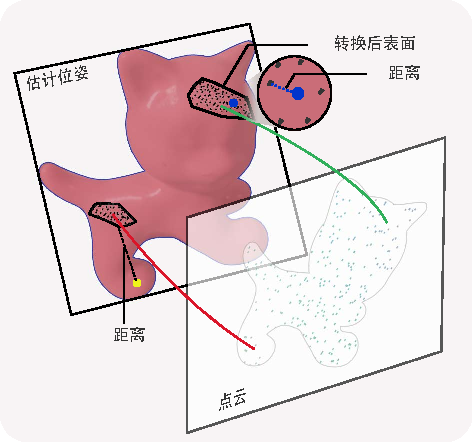
\includegraphics[width=0.5\textwidth]{figure/hipose/outlier_rejection.pdf}
    \caption{层次化对应关系剪枝策略}
    \label{fig:outlier_rejection}
\end{figure}

子表面划分和位姿估计重复 $n$ 次(从第 $m + 1$ 位到第 $d$ 位)。在第 $it$ 次迭代中,$it \in [0,1,...,n-1]$,计算点云中每个点 $\bm{P}$ 对应子表面的质心 $\bm{g}_{it}$,并通过 Kabsch 求解器估计此步骤中的位姿 $[\hat{\bm{R}}_{it}|\hat{\bm{t}}_{it}]$。利用此估计的位姿,使用下面计算的距离选择内点。

在第 $(it+1)$ 次迭代中,计算点 $\bm{P}$ 和在位姿 $[\hat{\bm{R}}_{it}|\hat{\bm{t}}_{it}]$ 下变换的子表面 $\bm{S}_{m+it}'$ 之间的每个对应关系的距离,该距离将用作区分内点和外点的阈值。\autoref{fig:outlier_rejection} 是此过程的可视化表示。
点云中点 $\bm{P}$ 和变换表面 $\bm{S}_{m+it}'$ 之间的最小距离定义为:
\begin{equation}
\label{eq:l}
l = \min\limits_{\bm{v}_i} ||\hat{\bm{R}}_{it} \bm{v}_{i} + \hat{\bm{t}}_{it}-\bm{P}||
\end{equation}

内点和外点的区分基于距离 $l$ 的中位数。不同的区分内点和外点的方法在消融实验中进行了比较,见\autoref{sec:exp}。形式上,在一般情况下,第 $it$ 次迭代的位姿通过 Kabsch算法求解,算法输入为点到表面质心的3D-3D对应关系集:
\begin{equation}
    \label{eq:posekabsch}
    [\hat{\bm{R}}_{it}|\hat{\bm{t}}_{it}] = {Kabsch}(\{\bm{P}_{k}, \bm{g}_{m+it}^{k}\}), {\bm{P}_{k}\in \text{inliers}_{it}}
\end{equation}

在完成 $n$ 次表面划分迭代后,所有点到面的对应关系都已收敛为点到点的对应关系。最后,使用所有在层次化对应关系剪枝过程中从未被识别为离群点的点到点对应关系进行一轮 Kabsch 算法,以生成最终估计的位姿 $[\hat{\bm{R}}_{n}|\hat{\bm{t}}_{n}]$。
